\section{Problem formulation}\label{sec:perceptionDistortion}

In statistical terms, a natural image $x$ can be thought of as a realization from the distribution of natural images~$p_X$. In image restoration, we observe a degraded version $y$ relating to $x$ via some conditional distribution $p_{Y \vert X}$. In this paper we focus on non-invertible settings\footnote{\label{foot:invertible}By invertible we mean that the support of $p_{X|Y}(\cdot|y)$ is a singleton for almost all $y$'s (see Appendix \ref{ap:distortionProofNonunique} for a formal definition).}, where $x$ cannot be estimated from $y$ with zero error. This is typically the case in denoising, deblurring, inpaitning, super-resolution, etc. Given $y$, an image restoration algorithm produces an estimate $\hat{x}$ according to some distribution $p_{\hat{X}\vert Y}$. Note that this description is quite general in that it does not restrict the estimator $\hat{x}$ to be a deterministic function of $y$. This problem setting is illustrated in Fig.~\ref{fig:problemSetting}.

\begin{figure}
	\begin{center}
		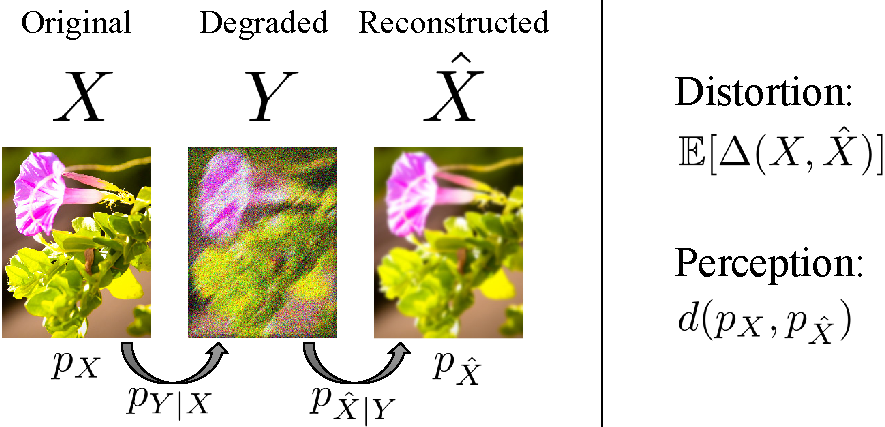
\includegraphics[width=0.9\linewidth]{figures/problemSetting3.pdf}
	\end{center}
	\caption{\textbf{Problem setting.} Given an original image $x\sim p_X$, a degraded image $y$ is observed according to some conditional distribution $p_{Y \vert X}$. Given the degraded image $y$, an estimate $\hat{x}$ is constructed according to some conditional distribution $p_{\hat{X} \vert Y}$. Distortion is quantified by the mean of some distortion measure between $\hat{X}$ and $X$. The perceptual quality index corresponds to the deviation between $p_{\hat{X}}$ and $p_X$.}
	\label{fig:problemSetting}
\end{figure}


Given a full-reference dissimilarity criterion $\Delta(x,\hat{x})$, the average distortion of an estimator $\hat{X}$ is given by
\begin{equation}\label{eq:AverageDistortion}
\E[\Delta(X,\hat{X})],
\end{equation}
where the expectation is over the joint distribution $p_{X,\hat{X}}$. This definition aligns with the common practice of evaluating average performance over a database of degraded natural images. We assume that the dissimilarity criterion is such that $\Delta(x,\hat{x}) \ge 0$ with equality when $\hat{x} = x$. Note that some distortion measures, \eg SSIM, are actually \emph{similarity} measures (higher is better), yet can always be inverted (and shifted) to become dissimilarity measures.

As discussed in Sec.~\ref{sec:RelatedWorkPerceptualQuality}, the perceptual quality of an estimator $\hat{X}$ (as quantified \eg by real vs.~fake human opinion studies) is directly related to the distance between the distribution of its reconstructed images, $p_{\hat{X}}$, and the distribution of natural images, $p_X$. We thus define the perceptual quality index (lower is better) of an estimator $\hat{X}$ as
\begin{equation}\label{eq:PerceptualQualityIndex}
d(p_X,p_{\hat{X}}),
\end{equation}
where $d(p,q)$ is some divergence between distributions that satisfies $d(p,q) \ge 0$ with equality if $p=q$, \eg the KL divergence, TV distance, Wasserstein distance, etc. It should be pointed out that the divergence function $d(\cdot,\cdot)$ which best relates to human perception is a subject of ongoing research. Yet, our results below hold for (nearly) any divergence.

Notice that the best possible perceptual quality is obtained when the outputs of the algorithm follow the distribution of natural images (\ie $p_{\hat{X}}=p_X$). In this situation, by looking at the reconstructed images, it is impossible to tell that they were generated by an algorithm. However, not every estimator with this property is necessarily accurate. Indeed, we could achieve perfect perceptual quality by randomly drawing natural images that have nothing to do with the original ground-truth images. In this case the distortion would be quite large.%.

Our goal is to characterize the tradeoff between \eqref{eq:AverageDistortion} and~\eqref{eq:PerceptualQualityIndex}. But let us first see why minimizing the average distortion \eqref{eq:AverageDistortion}, does not necessarily lead to a low perceptual quality index \eqref{eq:PerceptualQualityIndex}. We start by illustrating this with the square-error distortion $\Delta(x,\hat{x})=\|x-\hat{x}\|^2$ and the $0-1$ distortion $\Delta(x,\hat{x})=1-\delta_{x,\hat{x}}$ (where $\delta$ is Kronecker's delta). We specifically illustrate that those measures are generally not distribution preserving in the following sense.
\begin{definition}
We say that a distortion measure $\Delta(\cdot,\cdot)$ is \emph{distribution preserving} at $p_{X,Y}$ if the estimator $\hat{X}$ minimizing the mean distortion \eqref{eq:AverageDistortion} satisfies $p_{\hat{X}}=p_X$.
\end{definition}
More details about those examples are provided in Appendix~\ref{ap:MMSE-MAP} (Supplementary Material). We then proceed to discuss this phenomenon for arbitrary distortions in Sec.~\ref{sec:arbitrary_dist}.


\subsection{The square-error distortion}\label{subsec:MMSEMAP}
The minimum mean square-error (MMSE) estimator is given by the posterior-mean $\hat{x}(y)=\E[X|Y=y]$. Consider the case $Y=X+N$, where $X$ is a discrete random variable with probability mass function
\begin{equation}\label{eq:XdiscreteExample}
	p_X(x) =
	\begin{cases}
	p_1 \quad \quad x= \pm 1,\\
	p_0 \quad \quad x=0,
	\end{cases}
\end{equation}
and $N \sim \mathcal{N}(0,1)$ is independent of $X$ (see Fig.~\ref{fig:exampleMAP}). In this setting, the MMSE estimate is given by
\begin{align}\label{eq:xMMSE}
\hat{x}_{\text{MMSE}}(y)&= \sum_{n\in\{-1,0,1\}}n \,\,p(X=n|y),
\end{align}
where
\begin{equation}\label{eq:PosteriorDiscrete}
p(X=n|y) = \frac{p_n \exp\{-\frac{1}{2}(y-n)^2\}}{\sum_{m\in\{-1,0,1\}}\limits p_m \exp\{-\frac{1}{2}(y-m)^2\}}.
\end{equation}
Notice that $\hat{x}_{\text{MMSE}}$ can take any value in the range $(-1,1)$, whereas $x$ can only take the discrete values $\{-1,0,1\}$. Thus, clearly, $p_{\hat{X}_{\text{MMSE}}}$ is very different from $p_X$, as illustrated in Fig.~\ref{fig:exampleMAP}. This demonstrates that minimizing the MSE distortion \emph{does not} generally lead to $p_{\hat{X}}\approx p_{X}$.



\begin{figure}
	\begin{center}
        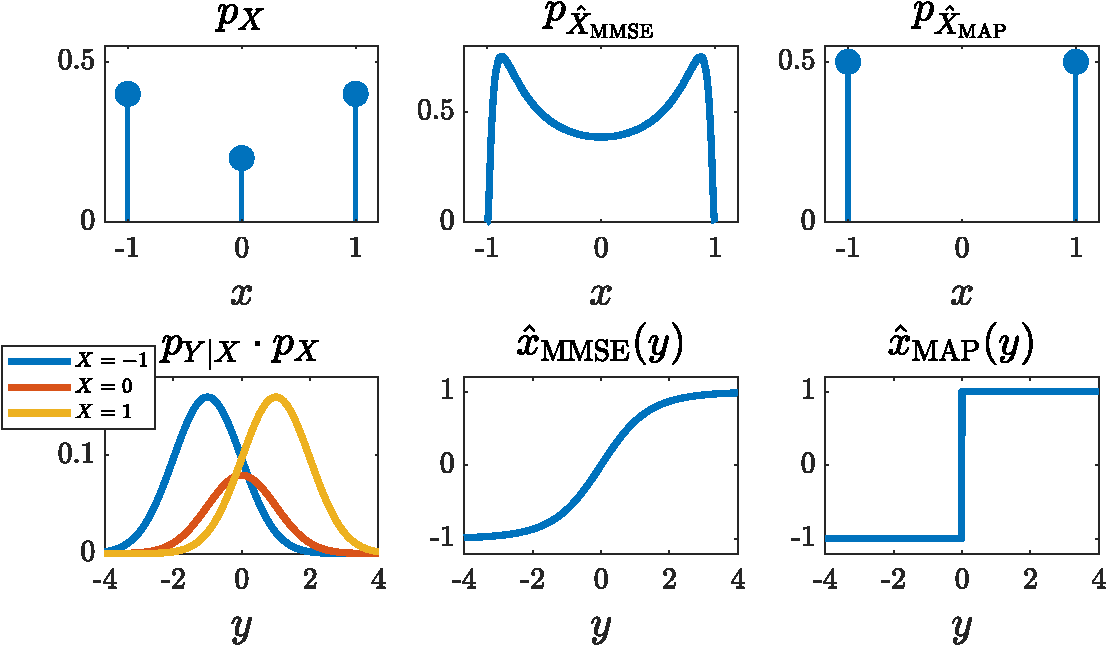
\includegraphics[width=\linewidth]{figures/exampleMAP.pdf}
	\end{center}
	\caption{\textbf{The distribution of the MMSE and MAP estimates.} In this example, $Y=X+N$, where $X \sim p_X$ and $N \sim \mathcal{N}(0,1)$. The distributions of both the MMSE and the MAP estimates deviate significantly from the distribution $p_X$.}
	\label{fig:exampleMAP}
\end{figure}


The same intuition holds for images. The MMSE estimate is an average over all possible explanations to the measured data, weighted by their likelihoods. However the average of valid images is not necessarily a valid image, so that the MMSE estimate frequently ``falls off'' the natural image manifold \cite{ledig2016photo}. This leads to unnatural blurry reconstructions, as illustrated in Fig.~\ref{fig:MMSE_MAP}. In this experiment, $x$ is a $280 \times 280$ image comprising $100$ smaller $28 \times 28$ digit images. Each digit is chosen uniformly at random from a dataset comprising $54$K images from the MNIST dataset \cite{MNIST} and an additional $5.4$K blank images. The degraded image $y$ is a noisy version of $x$. As can be seen, the MMSE estimator produces blurry reconstructions, which do not follow the statistics of the (binary) images in the dataset.


\begin{figure}
	\begin{center}
		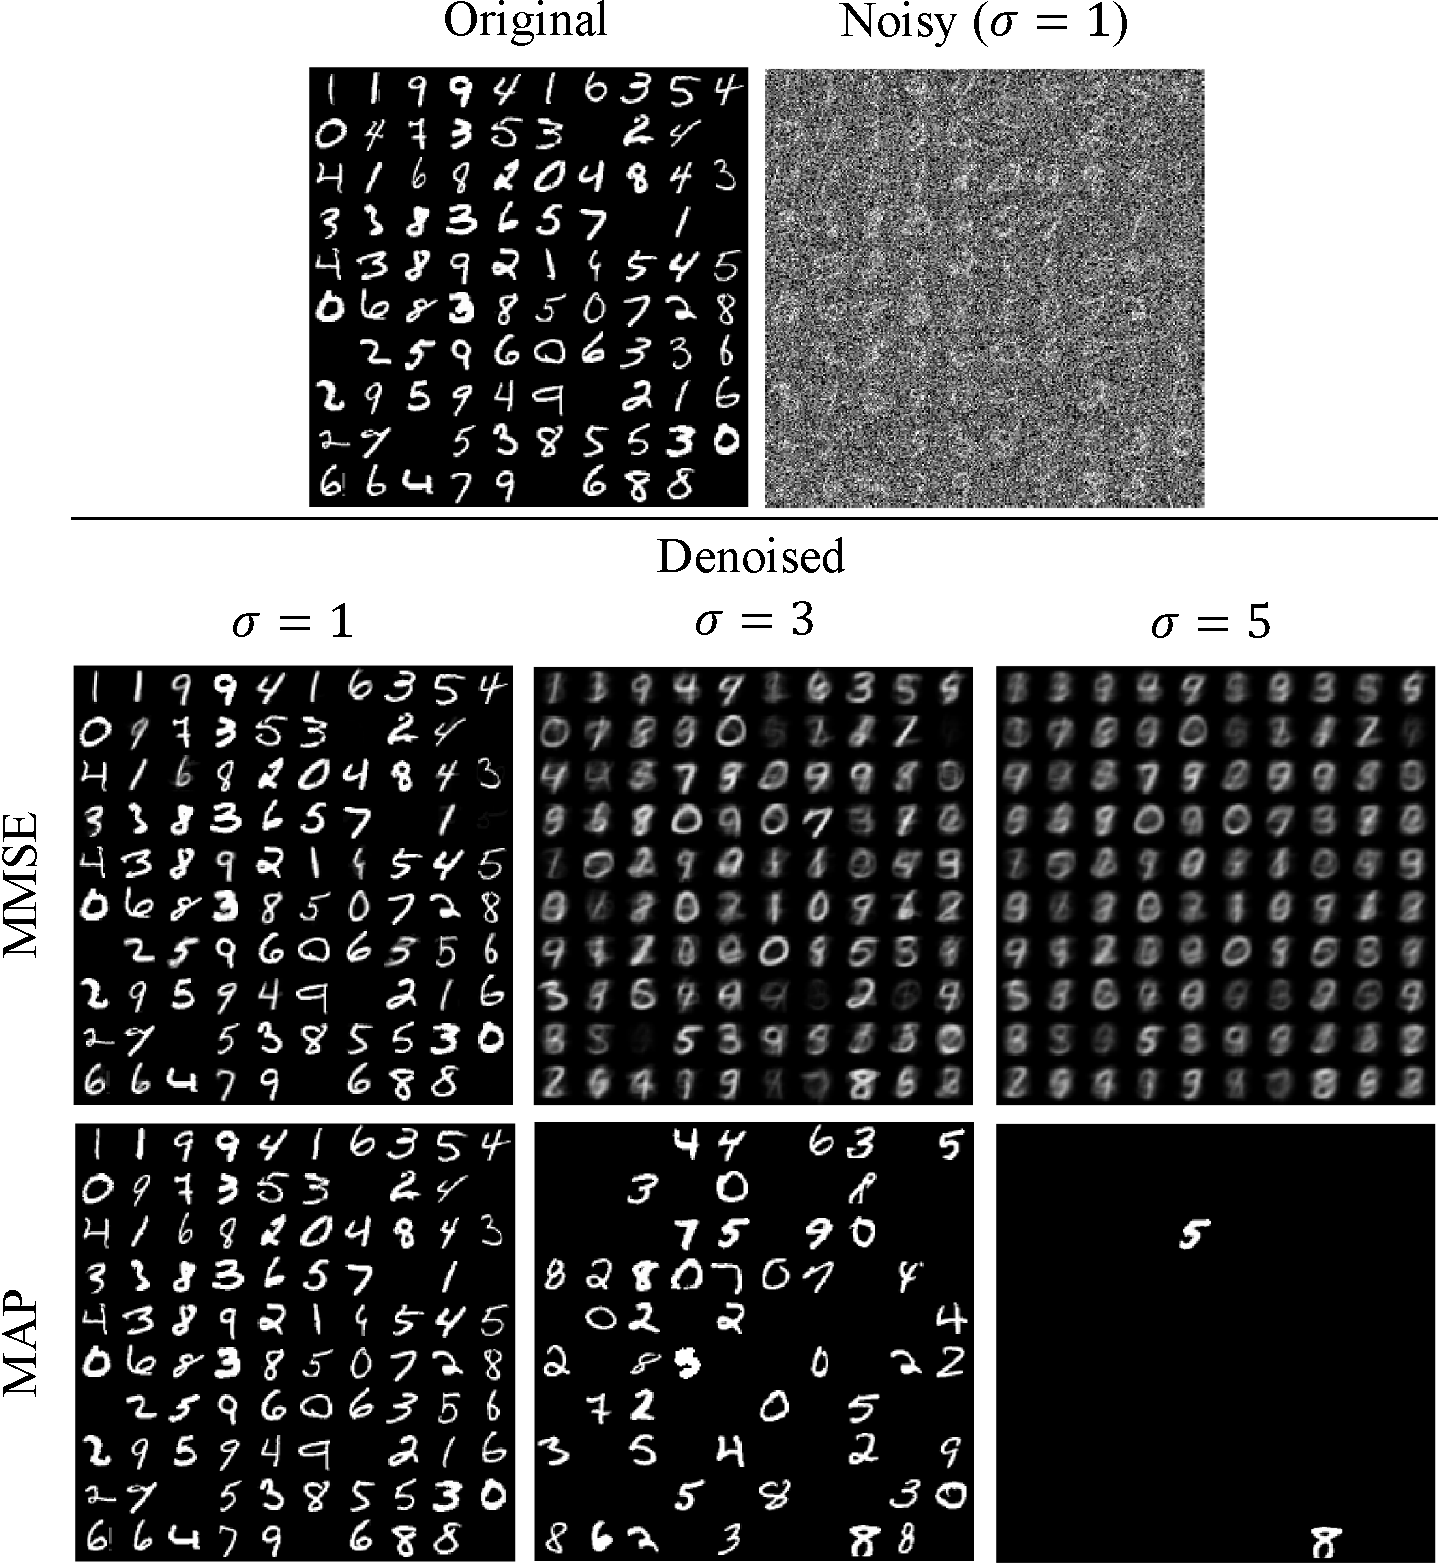
\includegraphics[width=0.93\linewidth]{figures/MMSE_MAP.pdf}
	\end{center}
	\caption{\textbf{MMSE and MAP denoising.} Here, the original image consists of $100$ smaller images, chosen uniformly at random from the MNIST dataset enriched with blank images. After adding Gaussian noise ($\sigma=1,3,5$), the image is denoised using the MMSE and MAP estimators. In both cases, the estimates significantly deviate from the distribution of images in the dataset.}
	\label{fig:MMSE_MAP}
\end{figure}

\subsection{The $0-1$ distortion}\label{subsec:MMSEMAP2}
The discussion above may give the impression that unnatural estimates are mainly a problem of the square-error distortion, which causes averaging. One way to avoid averaging, is to minimize the binary $0-1$ loss, which restricts the estimator to choose $\hat{x}$ only from the set of values that $x$ can take. In fact, the minimum mean $0-1$ distortion is attained by the maximum-a-posteriori (MAP) rule, which is very popular in image restoration. However, as we exemplify next, the distribution of the MAP estimator also deviates from $p_X$. This behavior has also been studied in~\cite{nikolova2007model}.

Consider again the setting of \eqref{eq:XdiscreteExample}. In this case, the MAP estimate is given by
\begin{align}
\hat{x}_{\text{MAP}}(y)&= \argmax_{n\in\{-1,0,1\}}\limits p(X=n|y),
\end{align}
where $p(X=n|y)$ is as in \eqref{eq:PosteriorDiscrete}. Now, it can be easily verified that when $\log(p_1/p_0)>1/2$, we have $\hat{x}_{\text{MAP}}(y)=\text{sign}(y)$. Namely, the MAP estimator never predicts the value~$0$. Therefore, in this case, the distribution of the estimate is
\begin{equation}
	p_{\hat{X}_{\text{MAP}}}(\hat{x}) =
	\begin{cases}
	0.5 \quad \quad \hat{x}=+1,\\
	0.5 \quad \quad \hat{x}=-1,
	\end{cases}
\end{equation}
which is obviously different from $p_X$ of \eqref{eq:XdiscreteExample} (see Fig.~\ref{fig:exampleMAP}).

This effect can also be seen in the experiment of Fig.~\ref{fig:MMSE_MAP}. Here, the MAP estimates become increasingly dominated by blank images as the noise level rises, and thus clearly deviates from the underlying prior distribution.

\subsection{Arbitrary distortion measures}\label{sec:arbitrary_dist}
We saw that neither the square-error nor the $0-1$ loss are distribution preserving. That is, their minimization does not generally lead to $p_{\hat{X}}=p_X$ (\ie perfect perceptual quality). However these two examples do not yet preclude the existence of a distribution preserving distortion measure. Does there exist a measure whose minimization is guaranteed to lead to $p_{\hat{X}}=p_X$? If we limit ourselves to one single setting, then the answer may be positive. For example, in the setting of Fig.~\ref{fig:exampleMAP}, if $p_0$ of \eqref{eq:XdiscreteExample} equals~$0$, then the $0-1$ loss is distribution preserving as its minimization leads to an estimate satisfying $p_{\hat{X}}=p_X$. This illustrates that a distortion measure may be distribution preserving for certain underlying distributions $p_{X,Y}$ but not for others.

However, from a practical standpoint, we typically want our distortion measure to be adequate in more than one single setting. For example, if our goal is to train a neural network to perform denoising, then it is reasonable to expect that the same distortion measure be equally adequate as a loss function for different noise levels. In fact, we may also want to use the same distortion measure across different tasks (\eg super-resolution, deblurring, inpainting). The interesting question is, therefore, whether there exists a \emph{stably} distribution preserving distortion measure.
\begin{definition}
We say that a distortion measure $\Delta(\cdot,\cdot)$ is \emph{stably distribution preserving} at $p_{X,Y}$ if it is distribution preserving at all $\tilde{p}_{X,Y}$ in a TV $\varepsilon$-ball around $p_{X,Y}$ for some $\varepsilon>0$.
\end{definition}

As we show next, if the degradation is non-invertible, then no distortion metric can be stably distribution preserving (see proof in Appendix~\ref{ap:distortionProofNonunique}).
\begin{theorem}\label{thm:arbitraryDistortion}
	If $p_{X,Y}$ defines a non-invertible degradation, then $\Delta(\cdot,\cdot)$ is not a stably distribution preserving distortion at $p_{X,Y}$.
\end{theorem}
